


%%%%%%%%%%%%%%%%%%%%%%%%%%%
\chapter {Black Virus Disinfection in Consecutive-Chord Rings}
\label{CL}
%%%%%%%%%%%%%%%%%%%%%%%%%%%
 


In this chapter, the black virus disinfection problem is considered in the {\it consecutive chord}  ring $C_n(1,2,3,..,k-1,k)$, with  $k < \lfloor\frac{n}{2}\rfloor$,  in a {\it synchronous} environment. 

% We remind that the {\it consecutive chords}  ring  is an interconnected ring of $n$ nodes $v_0, \ldots v_{n-1}$, where each node is connected to $2k$  neighbours: $k$ consecutive neighbours in each direction. 
% So, the neighbourhood of node $v_i$ is given by: $N(v_{i})=\{v_{i+1}$, $v_{i+2}$,..., $v_{i+k-1}$, $v_{i+k}$, $v_{i-1}$, $v_{i-2}$,..., $v_{i-k+1}$, $v_{i-k}\}$.




For the deployment phase, unlike the other classes of chordal rings, the local strategy that we propose, the {\it One-Direction Greedy} strategy,  is also a move-optimal solution. We thus only concentrate on local deployment.
As usual, we evaluate the complexity of the solution
 by considering the  overall number of agents employed, the number of agent casualties and the number of moves required.   The following table summarizes some of the results. 

 

\begin{center}
\scalebox{0.9}{%
  \begin{tabular}{|c|c|c|}
 \hline
   Consecutive-Chords(C)      & $|S_{area}\ge k$ & $|S_{area}< k$     \\

 \hline
 Spread(C)   &  $\leq k+1 $  &$ \leq 2k$  \\ 
 \hline
 Size(C)   &  $\leq 3k+1$ &  $\leq 4k+2$\\
 \hline
Move(C)   & $\leq (k+3)n-(\frac {3k^2+5k}{2} )$ & $\leq k(\lceil \frac {n-k-1}{k} \rceil) +6k$ \\
 \hline
 \end{tabular}}
 \end{center}
%\leq (3n-k-5)+(\sum\limits_{i=2}^{k} n-k-1-i) + k(\lceil \frac {n-k}{k} \rceil) (k+3)n-(\frac {3k^2+5k}{2} )-3






\section{Exploration and Shadowing}

The exploration phase is the same as in all the other chordal rings. We instantiate it here for the particular case of the consecutive-chords chordal ring.

 
\begin{center}
\fbox{
\begin{minipage}{6cm}
{\sc  Exploration and Shadowing}
  \begin{tabbing}
Let \=  $HB= v_0$.   Agents $EA $ and $$LEA$$ at safe node  $v_j$.\\
\\
if  $j<k$  (*  $N_{ex}(v_j) = \{ v_{j-1},v_{j-2},...,v_{0}\}$ *) \\
\>    $ (j-1)  SH$s are deployed to protect $N_{ex}(v_j)$ \\
Else if  $k\leq j < n-k$  (*  $N_{ex}(v_j) = \{ v_{j-1},v_{j-2},v_{j-3},...,v_{j-k} \}$ *) \\  
\>    $k-1$ $SH$s are deployed to protect $N_{ex}(v_j)$ \\
 Else if  $n-k \leq j \leq n-1$  (* $N_{ex}(v_j) = \{ v_{j-1},v_{j-2},\ldots, v_{j-k} ,v_{j+k},v_{j+k-1}, \ldots, v_{0}\}$ *) \\
\> let $j=n-i$, where $i \in \mathbb{Z}_{\geq 0}$ {\bf why this line ? j is already defined, isn't it ?} \\
{\bf here at this segment the value of j would be n- some value  i,}\\
 {\bf I think we need to state that so we can understand where i comes from}\\
\>   ($2k-i$) $SH$s are deployed to protect $N_{ex}(v_j)$ \\
 EA moves to $v_{j+1}$.\\ 
 \end{tabbing}
\end{minipage}
}
\end{center}


 
The observations below were obtained following the application of this strategy:



\begin{theorem}
In the worst case scenario, the {\em exploration and shadowing phase}
ends with the triggering of the \bv in $(k+2)n-2k-3$ moves.
%$(3n-5)+(\sum\limits_{i=2}^k n-1-i)+ (\sum\limits_{i=1}^{k-1}i)$
\end{theorem}
\begin{proof}
The worst case scenario for the number of moves required occurs when the \bv  is found at node ($v_{n-1}$) after exploring $n-1$ nodes.  
  In this case, the $BV$ triggers no new \bvs since all of the neighbouring nodes in the safe area have been explored and are protected by $SH$s.
The complexity of this case is  $3(n-1)-2$ for the movement of $LEA$ and $EA$, $(\sum\limits_{i=2}^k n-1-i)$ for the movement of $k-1$ $SH$s in the counter clockwise direction and $(\sum\limits_{i=1}^{k-1}i)$ for the movement of  $SH$s in the other direction.
{\bf here you don't explain how you come up with that summation By the way, are the SH created when needed, or do they go directly from the HB ? We have to be consistent with what we did in the rest. If they go from the HB, I don't see the need of the summation.}\\
{\bf  SHs always created at the begining then they have timers that synchronize their movements with the exploring team, yes we need the summation since SHs walking in a consecutive manner following LEA}
\end{proof}
%

%
\begin{theorem}
In any consecutive chord ring, the maximum number of \bvs created after triggering the original one is $(2k-1)$.

\end{theorem}

\begin{proof}
The worst case scenario for the number of \bvs created upon activating the original \bv is when the original is found at node $v_i$ where $\leq i =1$. In this case, the \bv ($x_0$)  triggers ($2k-1$) new {\it black viruses}:  $x_1$, $x_2$, $x_3$, ..., $x_k$, and  $x_{-2}$, $x_{-3}$, ..., $x_{-k}$ because no $SH$ have been deployed. Note that  $x_{-1} $ is always occupied by $LEA$.

\end{proof}
%%%%%%%%%%%%%%%%%








\section{Surrounding and Eliminating}


The deployment phase of the consecutive chords chordal ring is different from all the other structures considered in this thesis because when the \bv is triggered, the chordal ring gets disconnected. 
 
% As usual,  let $x_0$ be the original $BV$, node $x_{-1}$ is always protected by $LEA$ while  the other neighbours are  protected only if they belong to the safe area and are occupied by shadow agent(s), $SH$; otherwise, they are affected depending on their location.
%Summarizing, in the best case in term of the number of {\it black viruses}, after $EA$ triggers the original black virus, no more $BV$s are created, while the worst case, $2k-1$ $BV$s are created.  \\
%To handle the spread of the $BV$s, $LEA$ has to send agents to surround and clear those faults. 
%
%To do so, $LEA$ creates agents to be sent to specific targets (i.e., neighbours of \bvs), and after all agents are at their positions, $LEA$ sends cleaning agents, $CA$s to trigger all the $BV$s at once, so we need as many $SA$s as the neighbours of the $BV$s and as many $CA$s as the $BV$s. 
%
%
%First, we remind some notation.   
%Let $x_0$ be the discovered BV.
% We denote by  ${\cal BV}$ the set of black viruses in the system.
% Let ${\cal S} = V - {\cal BV}$ be  the set of the  clean nodes not containing any $BV$. Let 
%  ${\cal T}$ be  the set of targets, that is the nodes to be occupied. Let $S_{area}$ be the {\it safe area}, and  $\left\vert{S_{area}}\right\vert$ is the number of nodes in that area.  Let $D_{area}$ be the {\it danger area} where recontamination need to be avoided.



  \begin{center}
\fbox{
\begin{minipage}{8.5cm}
{\sc Surrounding and Elimination} 
  \begin{tabbing}
   $$LEA$$ \= and  $SH$s  covering all $N_{ex}(v)$ \\ \\
   
   
 $BV$ comes back from $v=x_0$. \\ 

 if ($|S_{area}|=1$) \\
\tab(*  $$LEA$$ is covering $x_{-1}$ *) \\

  \tab   $N_{un}(x_0) =\{x_{1},x_{2},...,x_{k},x_{-2},x_{-3},..., x_{-k+1},x_{-k} \}$ \\ 

 if ($1<|S_{area}|<k$)\\ 

\tab let $|S_{area}|=k-i$, where $i \in \mathbb{Z}_{\geq 0}$ \\
\tab(*  $$LEA$$ is covering $x_{-1}$ and $SH$s covering $N_{ex}(x_0)$*) \\
  \tab   $N_{un}(x_0) =\{x_{1},x_{2},..., x_{k},x_{-k},x_{-k+1},x_{-k+2},..., x_{-k+i-1} \}$ \\ \\

if  ($k\leq |S_{area}| <n-k$) \\

 \tab(*   $$LEA$$ \= and  $SH$  covering $x_{-1},x_{-2},...,x_{-k}$ *) \\
  \tab  $N_{un}(x_0) =\{x_{1},x_2,...,x_{k}\}$  \\ \\

if  ($n-k\leq |S_{area}| <n-1$) \\

\tab let $|S_{area}|=n-i$, where $i \in \mathbb{Z}_{\geq 0}$ \\
\tab(*  $$LEA$$ \= and  $SH$s  covering $x_{-1},x_{-2},...,x_{-k}, x_{i},x_{i+1},...,x_{k}$ *)\\
  \tab  $N_{un}(x_0) =\{x_{1},x_{2},...,x_{i-1}\}$  \\ \\

Else \\
 \tab(*  $$LEA$$ \= and  $SH$s  covering $x_{-1},x_{-2}...,x_{-k},x_1,x_{2},...,x_{k}$ *)\\
  \tab  $N_{un}(x_0) =\emptyset $ \\ \\

   \\
 All $SH$ make one move in  clockwise direction.\\ %when they receive bv, they make 1 move and  stay there
 For \= each $u \in   N_{un}(x_0)$:\\
\>  {\sc Deploy}  an  agent   to each  $z\in \{N(u)\setminus  N_{un}(x_0)\}$\\

  Wh\=en $N(u)$ is covered:\\
 \> {\sc Deploy} one agent to   $u$
  \end{tabbing}
\end{minipage}
}
\end{center}


% From the previous algorithm, notice that once a $SH$ receives a {\it black virus}, it moves to the neighbouring node through chord $+1$ in order to be part of the surrounding team. Thus, we can see that sometimes agents change their roles. 
%
%We remind that in this model we assume synchronicity, so all agents are synchronized and it takes one time unit   to traverse a link connecting two neighbouring nodes. 

As with the previous chapters, we will consider different cases depending on the location of the \bv.
More precisely, the number of agents required to disinfect the consecutive-chords ring $C_n$ depends entirely on the chord structure and the location of black viruses in respect to the safe area. We first  partition the chordal ring into four distinct segments using $v_0$ as the home base.

\begin{itemize}
\item {\em Segment 1} contains node $v_1$.  
If the \bv is in this segment, the size of the safe area is $|S_{area}| =1$.
%:  $1\leq i <k$
\item {\em  Segment 2} contains nodes $v_2, \ldots v_{k-1}$.   If the \bv is in this segment, the size of the safe area is $|S_{area}| =k-2$.
\item {\em   Segment 3} contains nodes $v_k, \ldots v_{n-k-1}$.   If the \bv is in this segment, the size of the safe area is $|S_{area}| =n-2k$.
%: $k\leq i <n-k$
\item {\em Segment 4}  contains nodes $v_{n-k}, \ldots v_{n-1}$.   If the \bv is in this segment, the size of the safe area is $|S_{area}| =k$.
%: $n-k\leq i \leq n-1$
\end{itemize}

 

%%\end{proof}

 
\begin{theorem}\label{theo:agents_cc}
For black virus disinfection in consecutive-chords ring $C_n(1,2,...,k)$, a maximum of $(4k+1)$ agents are employed.

\end{theorem}
\begin{proof}
The number of agents is determined according to the location of the original $BV$ and the chord structure.
\begin{itemize} 
\item
When the $BV$ is located at any node in  {\em Segment 1}, 
we have  the worst complexity in terms of $CA$ and $SA$ since activating the \bv will create $(2k-1)$ \bvs at $x_{1},x_{2},...,x_{k},x_{-2},x_{-3},...,x_{-k}$. Subsequently, the $LEA$ moves to $x_{0}$ and then deploys $2k$ while one $SH$ is created in the $x_{-1}$, which was the homebase.
%+1 for x_{-1}
The $SA$s are then to occupy $x_{k+1},x_{k+2},x_{k+3},...,x_{2k},x_{-k-1},x_{-k-2},...,x_{-2k}$. The total number of agents employed is then $(4k+2)$:  $(2k)$ $CA$s, $(2k)$  $SA$s, one $SH$ and one $LEA$. Therefore, $Spread(C)=2k$ and $Size(C)=4k+2$.   
 
\item If the $BV$ is located at any node in {\em  Segment 2 },
activating the original \bv would create $k+i$  \bvs at $x_{1}$, $x_{2}$,..., $x_{k}$, $x_{-k}$, $x_{-k+1}$ ,..., $x_{-k+i}$, where $i=k-|S_{area}|$. The same number of $SH$s as nodes in the safe area arethen deployed and each makes one move through $+1$ chord when it receives a $BV$. $LEA$ also moves to $x_{0}$, and then  deploys $2k$  $SA$s to occupy $x_{k+1}$, $x_{k+2}$, $x_{k+3}$, ..., $x_{2k}$, $x_{-k-1}$, $x_{-k-2}$, ..., $x_{-2k}$.
Therefore, the team of agents consists  of $(4k+2)$ agents: $(k+i+1)$ $CA$s, $(2k)$  $SA$s, $(|S_{area}|)$ $SH$s and $LEA$. In this case,  $Spread(C)=k+i+1=2k-|S_{area}|+1$ and $Size(C)=4k+2$.
%should we consider agent at node -1 a shadow or SA?????????


\item If the $BV$ is located at any node in {\em Segment 3},
activating the original \bv would create $k$  \bvs at $x_{1}$, $x_{2}$,..., $x_{k}$,  while the other neighbouring nodes are already guarded. Once the $LEA$ and $SH$s receive $BV$s, they make one move through their $+1$ chords. Then $LEA$  deploys $k$  $SA$s to occupy $x_{k+1},x_{k+2},x_{k+3},...,x_{2k}$.
Therefore, the team of agents consists  of $(3k+1)$ agents: $(k+1)$ $CA$s, $(k)$  $SA$s, $(k-1)$ $SH$s and $LEA$. In this case,  $Spread(C)=k+1$ and $Size(C)=3k+1$.
 
\item If the $BV$ is located at any node in {\em  Segment 4 }, also called  the {\it Danger area} ($D_{area}$), we have two possible cases:

\begin{itemize}
\item When $n-k \leq |S_{area}| < n-1$:
Let us assume that $|S_{area}|=n-i$.
If the $BV$ is located at any node in this segment, activating the original \bv would create $i-1$ \bvs at $x_{1}$, $x_{2}$,..., $x_{i-1}$, while the other neighbouring nodes are guarded by $SH$s. In addition to the $SH$s at $x_{-1}$, $x_{-2}$,..., $x_{-k}$, $x_{i}$, $x_{i+1}$, $x_{i+2}$,..., $x_{k}$, and the $LEA$ at $x_{0}$, the $LEA$ deploys $i-2$  $SA$ to guard the unoccupied neighbours by $SH$s .
Therefore, the team of agents consists of $(2k+i-1)$ agents: $(i)$ $CA$s, $(i-2)$  $SA$, $(2k-i)$ $SH$ and $LEA$. In this case,  $Spread(C)=i=n-|S_{area}|$ and $Size(C)=2k+i-1=3k-|S_{area}|-1$.


\item When $|S_{area}|=n-1$:
No more \bvs are created  since all of the neighbouring nodes of the \bv are guarded by $SH$s and the $LEA$. No $SA$s to be deployed and all of the moves are made in the first phase. 
In this case,  the team consists of $2k+1$ agents: $1$ $CA$, $2k-1$ $SH$s and $LEA$. Therefore,$Spread(C)=1$ and $Size(C)=2k+1$.

\end{itemize}
\end{itemize}
\end{proof}

%\underline{\bf Revise the previous}


%% I should specify the unexplored neighbours in the previous algorithm and find a simple way %%to add it .

 
As previously mentioned, triggering the \bv disconnects the chordal ring and in order to reach the targets to surround the new black viruses, the agents must move in a counter-clockwise direction.


{\bf to discuss.}
The idea is for the surrounding agents to take the longest chord $-k$ to reach the area to be occupied as quickly as possible, and then reach their own target in one additional step through a shorter chord. 
Each agent can locally decide the following step  at each intermediate node, simply on the basis of its target.
 
 
% 
% For the deployment part, the optimal  routing approach is what we propose, the one-direction greedy strategy. Unlike other classes of chordal rings, there are no special paths that are irrelevant to the number of nodes nor to the chords structure since there is no way to reach  targets in the clockwise direction through $x_{-1}$. Also, the simple greedy does not work for the routing ; in fact it  causes infinite loops as in the triple loop and never does the routing correctly.
%Therefore,  we propose a strategy that adds some adjustments to the simple greedy approach. 
%In this topology, the only way  to clear all the $BV$s  is by wrapping around through the counter clockwise direction using the one-direction greedy algorithm and the decisions to reach  targets is made locally by the agents. 
%\begin{definition}
%The one-direction greedy routing is a greedy strategy that it only works in the counter clockwise direction causing the $SA$s to move from one node to another through only chord $-k$ until they reach a certain distance apart from their targets where they use the simple greedy approach.  
%\end{definition}
The one-direction greedy consists of two stages: the long jumps and the simple greedy. The long jumps portion forces $SA$s to move from $x_{0}$ to their targets through the edge($-k$) in a counter-clockwise direction making  $(\lceil  \frac {n-k}{k} \rceil -2)$ hops. At that point an extra hop will cause them to reach their destination.

{\bf "they start the simple greedy approach to reach their targets depending on the distances." Aren't they at distance 1 from their target now ?}





%%%%%%%%%%%%%%%%%%%%%%%%%%%%%%%%%%%%%%%%

\begin{comment}
{\bf I don't understand. To be discussed. Counting the jump is not really local anymore: you maintain info. Better to decide on the basis of the current location}
\begin{center}
\fbox{
\begin{minipage}{7.5cm}
{\sc One-direction Greedy}
\begin{tabbing}

Agent $A$ at node $x_{0}$\\
\tab If $|BV|\leq k$\\
  \tab Agent $A$ moves through  $\lambda=-k$  \\

\tab If $|BV|>k$\\
  \tab Agent $A$ moves through  $\lambda=-1$, then moves through $\lambda=-k$  \\

 $jump=1$\\

 If $jump=(\lceil  \frac {n-k}{k} \rceil -2)$ \\
\tab Depl\=oying agent $A$ arriving at $v$ from $y$ through $\lambda$ with destination $z$\\
 \tab Let $FD =\{ N(v)- {\cal BV} - y \}$ be the set of feasible destinations.\\
 \tab Agent $A$ moves to $w \in FD$ that minimizes $dist(w,z)$\\
 Else\\
 \tab Agent $A$ moves through  $\lambda=-k$  \\
 \tab Agent A calculates $jump++$  \\


\end{tabbing}
\end{minipage}
}
\end{center}
%%%%%%%%%%%%%%%%%%%%%%%%%%%%%%
%\tab Agent A calculates $Myloc= n+ \lambda$  \\
 %\tab Agent A calculates $Myloc= Myloc+ \lambda$  \\%%%%



%%%%%%%%%%%%%%%%%%%%%%%%%%%%%%%%%%%%%%%%
\end{comment}

{\bf indexes to be checked.}
\begin{center}
\fbox{
\begin{minipage}{7.5cm}
{\sc One-direction Greedy}
\begin{tabbing}
 Agent  $A$ at node $x_{-i}$ ($i\geq 0$) with target $x_j$ {\bf something like this.}\\

If $i=0$ \\
\tab If $|BV|\leq k$\\ 
  \tab \tab Agent $A$ moves through  $\lambda=-k$  \\

\tab If $|BV|>k$\\
  \tab \tab Agent $A$ moves through  $\lambda=-1$, then moves through $\lambda=-k$  \\

If $i < k(\lceil  \frac {n-k}{k} \rceil -2)$\\
\tab move through $\lambda=-k$\\
Else .... {\bf aren't we now one hope from the target ? yes}\\
\tab Let $FD =\{ N(v)- {\cal BV} - y \}$ be the set of feasible destinations.\\
 \tab Agent $A$ moves to $w \in FD$ that minimizes $dist(w,x_j)$\\

\end{tabbing}
\end{minipage}
}
\end{center}
%%%%%%%%%%%%%%%%%%%%%%%%%%%%%%




\begin{theorem}
In any consecutive chordal ring $C_n(1,2,3,...,k)$, with  $ k  < \lfloor\frac{n}{2}\rfloor$, using the one-direction greedy approach in the surrounding and eliminating phase disinfects the whole topology from {\it black viruses}.
\end{theorem}

\begin{proof}
After finding the original {\it black virus}, and depending on the size of the safe area, we get $BV$s in the clockwise direction or in both directions. In the first scenario we have $|S_{area}|\ge k$ and all $BV$s reside in one direction (clockwise). From the location of the $LEA$, the other direction is completely safe and clean,   and all agents can  traverse that part of the chordal ring until they reach their targets. In order to do so, the agents must be aware of the locations of $BV$s according to our algorithm. 
In the second scenario we have  $|S_{area}|< k$, $ k$$BV$s reside in the clockwise direction, and $\leq k$ $BV$s reside in the counter clockwise direction. From the location of the $LEA$ the counter clockwise direction is not quite as safe as it was in the first scenario. Agents can still traverse that direction safely due to the fact that the node $x_{-1}$ is always safe no matter the size of the safe area. 

Through node $x_{-1}$, the $LEA$ will send agents to their targets, and the agents will avoid all the faulty nodes in that direction since the longest chord connected to $x_{-1}$ surpasses the furthest possible $BV$ (i.e., $x_{-1-k} < x_{-k}$).

\end{proof}

In the following section we will consider the number of moves required  in the two main cases: $|S_{area}|\ge k$ and  $|S_{area}|< k$.
\begin{theorem}
In any consecutive chordal ring $C_n(1,2,3,...,k)$, with  $ k  < \lfloor\frac{n}{2}\rfloor$, when $|S_{area}|\ge k$, the number of moves required to surround and eliminate the {\it black viruses} is $\leq k(\lceil \frac {n-k}{k} \rceil) +2k$, regardless of the number of nodes.
\end{theorem}


\begin{proof}
The number of moves required to decontaminate $k BV$s can be calculated as follows:
\begin{itemize}
\item One move is made by $LEA$ to occupy $x_{0}$.
\item The movements of $SA$s are calculated as follows:
\begin{enumerate}
  \item Calculating the number of jumps. Agents need to traverse the ring starting from $x_{0}$ and using the longest chord as they move greedily: \begin{equation}\label{q1}
\lfloor \frac {n-k}{k} \rfloor 
\end {equation}
  \item Finding the number of $leftover$ nodes, which are not reached from the last jump, and require an extra jump:
 \begin{equation}\label{q2}
leftover=((n-k)\mod k ) -1 
\end {equation}   
This equation excludes BVs and $x_{0}$.
  
  \item Based on the aforementioned equations, we have the following information: 
\begin{itemize}

\item If \ref{q2}$\ge 0$, then $((n-k)\mod k ) -1$  neighbours are reached within $\lfloor \frac {n-k}{k} \rfloor  +1$,  
and $k- ( ((n-k)\mod k ) -1)$ neighbours are reached within $\lfloor \frac {n-k}{k} \rfloor  $. In total we have: \\
$(k- leftover) \lfloor \frac {n-k}{k} \rfloor + leftover (\lfloor \frac {n-k}{k} \rfloor  +1)$
\item If \ref{q2}$< 0 $, all neighbours except one are reached within $\lfloor \frac {n-k}{k} \rfloor $. The other neighbour is reached in $\lfloor \frac {n-k}{k} \rfloor -1$. In total, we have: \\
$(k-1)\lfloor \frac {n-k}{k} \rfloor + (\lfloor \frac {n-k}{k} \rfloor -1)$
% at most the number of moves for any case is $k\lfloor \frac {n-k}{k} \rfloor$
\end {itemize}
\end{enumerate}
In the theorem we substitute the floor function with the ceiling function in order to give a general upper bound for all of the possible values.

\item The $SH$s movements equal $k-1$  at most since all $SH$s make one move in the clockwise direction when the original \bv is activated.
\item $LEA$ sends $k$ $CA$s in $k$ moves to trigger the $BV$s.

\end{itemize}
\begin {center}
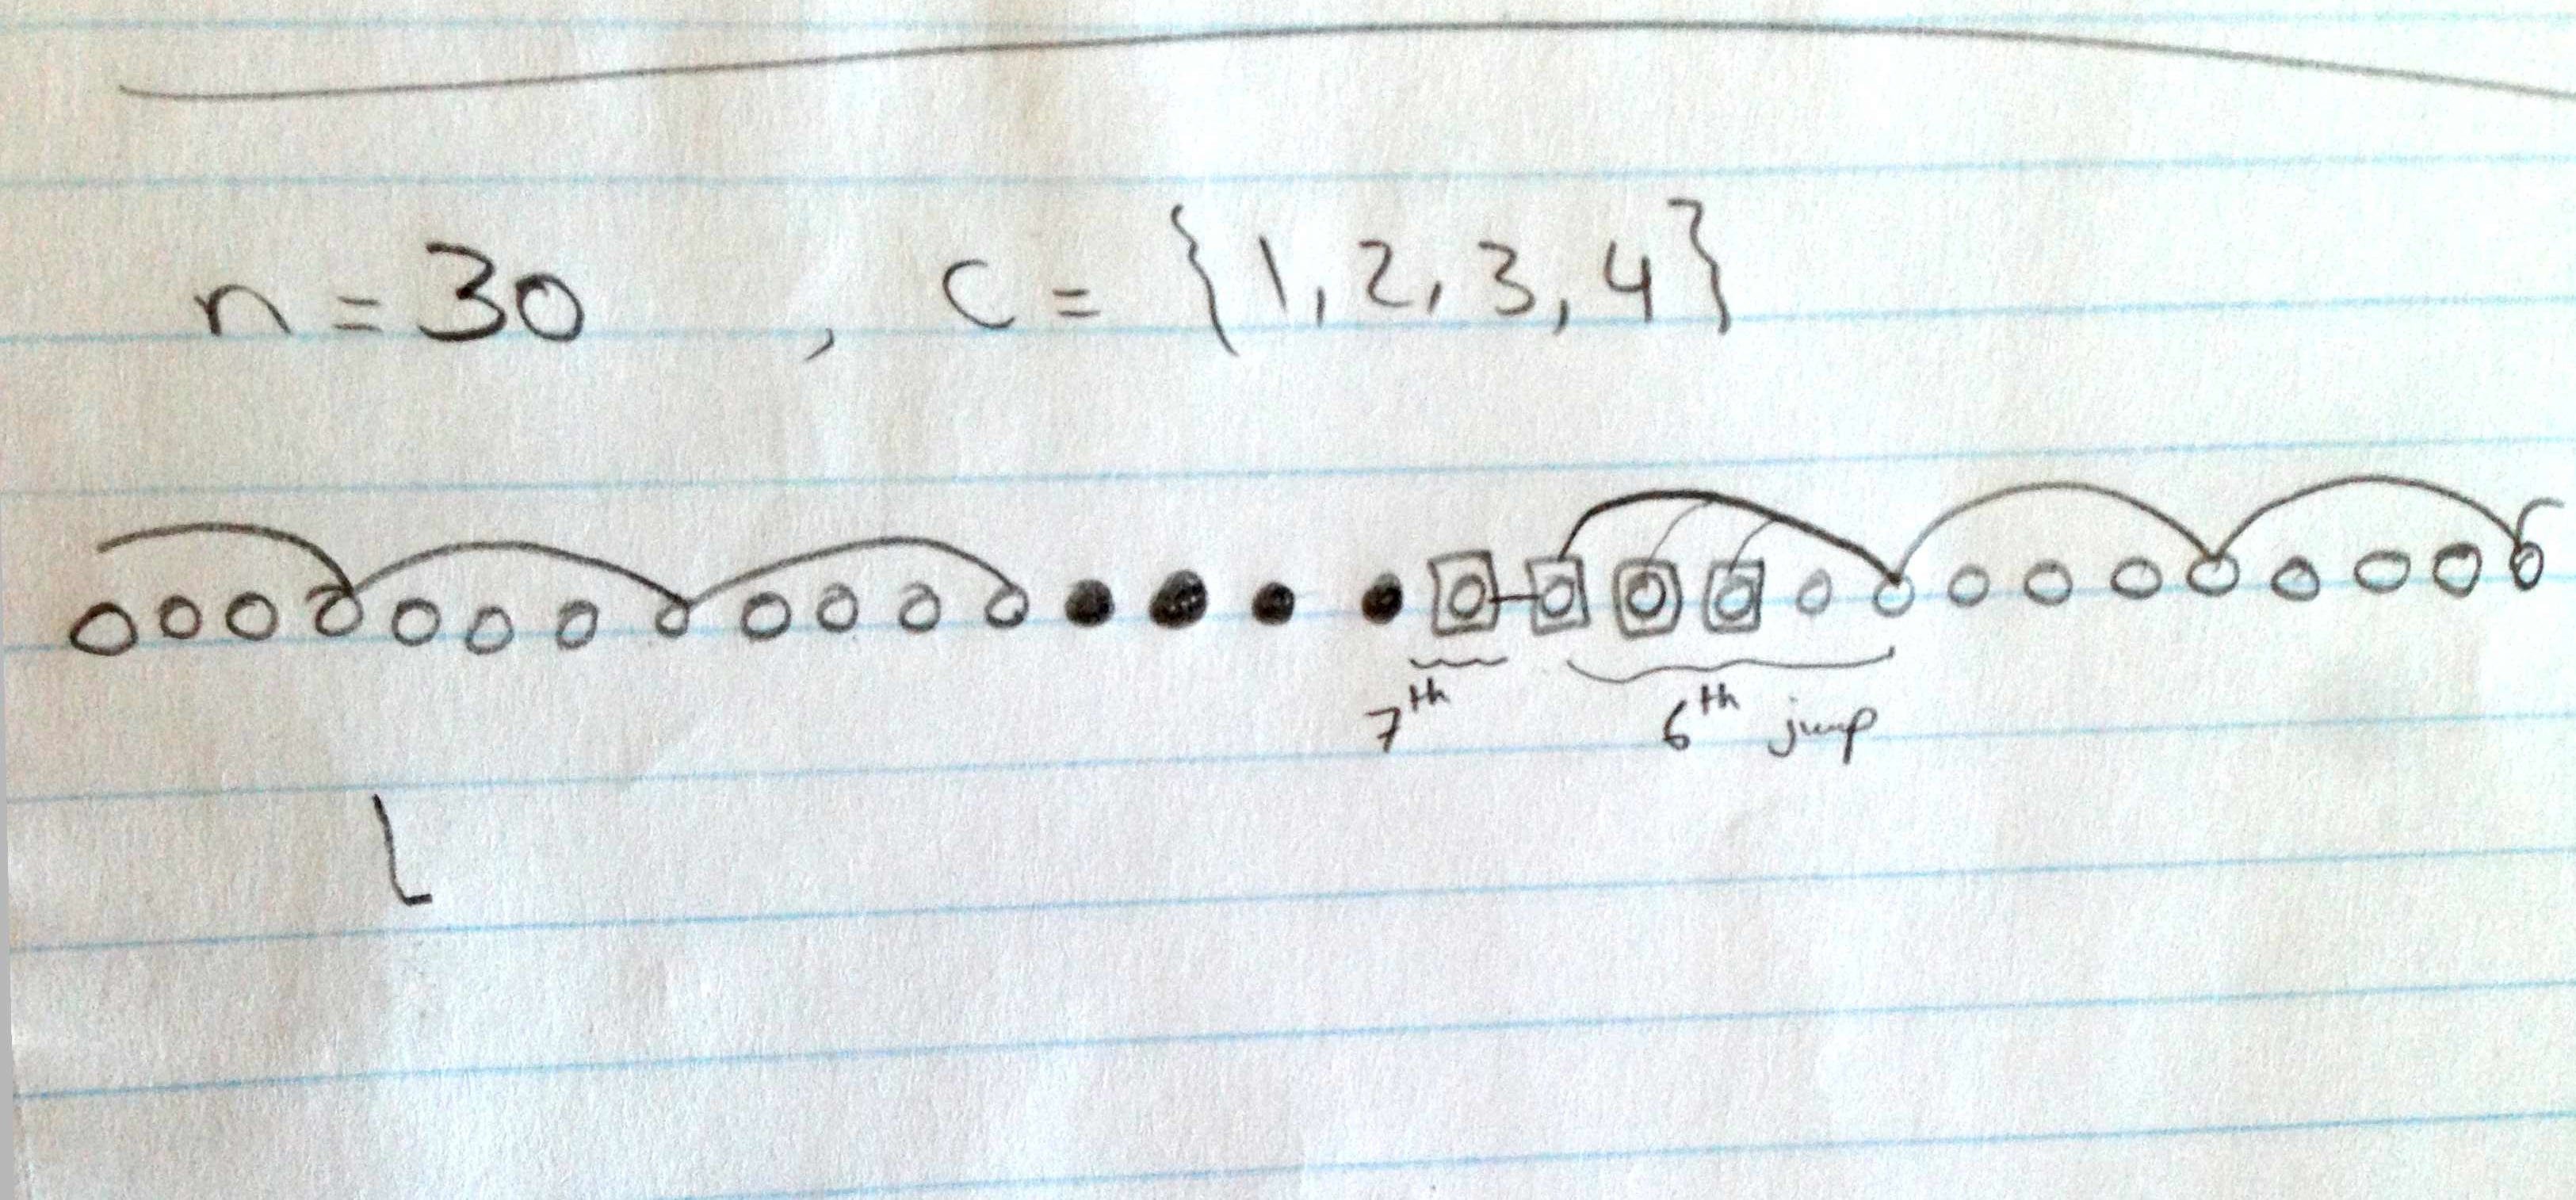
\includegraphics [scale=0.50] {consecutive.jpg}
\end {center}
\end{proof}




\begin{theorem}
In any consecutive chordal ring $C_n(1,2,3,...,k)$, with  $ k  < \lfloor\frac{n}{2}\rfloor$, when $|S_{area}|< k$, the number of moves required to surround and eliminate the {\it black viruses} is $\leq k(\lceil \frac {n-k-1}{k} \rceil) +6k-1$, regardless of the number of nodes.
\end{theorem}


\begin{proof}
The number of moves required to decontaminate the worst case scenario in terms of $spread$ and $size$ (i.e., when $|S_{area}|=1$) can be calculated as follows:
\begin{itemize}
\item One move is made by $LEA$ to occupy $x_{0}$.

In the worst case scenario we have $2k-1$ $BV$s, so in addition to $\{x_{k+1},x_{k+2},x_{k+3},...,x_{2k}\}$, there are more nodes to be guarded: $\{x_{-k-1},x_{-k-2},x_{-k-3},...,x_{-2k}\}$ The only way to reach those targets is through $x_{-1}$.

\item $k$ agents reach the  consecutive neighbours $\{x_{k+1},x_{k+2},x_{k+3},...,x_{2k}\}$ by wrapping around in the counter clockwise direction after moving from $x_{0}$ to $x_{-1}$ and using the one-direction greedy strategy. The movements of this group of  $SA$s are calculated in the same way as the previous case when $|S_{area}|\ge k$ except that the long jumps start from $x_{-1}$.




\begin{enumerate}
  \item Calculating the number of jumps. Agents need to traverse the ring starting from $x_{-1}$ and using the longest chord as they move greedily: \begin{equation}\label{q3}
\lfloor \frac {n-k-1}{k} \rfloor 
\end {equation}
  \item Finding the number of $leftover$ nodes, which are not reached from the last jump, and require an extra jump:
 \begin{equation}\label{q4}
leftover=((n-k-1)\mod k ) -1 
\end {equation}   
This equation excludes BVs and $x_{0}$.
  
  \item According to the aforementioned equations, we know that: 
\begin{itemize}

\item If \ref{q4}$\ge 0$, then $leftover$  neighbours are reached within $\lfloor \frac {n-k-1}{k} \rfloor  +1$,  
and ($k- leftover$) neighbours are reached within $\lfloor \frac {n-k-1}{k} \rfloor  $. In total, we have:\\
$$(k- leftover) \lfloor \frac {n-k-1}{k} \rfloor + leftover (\lfloor \frac {n-k-1}{k} \rfloor  +1)+k$$

\item If \ref{q2}$< 0 $, all neighbours except one are reached within $\lfloor \frac {n-k-1}{k} \rfloor $. The other neighbour is reached in $\lfloor \frac {n-k-1}{k} \rfloor -1$. In total, we have: \\
$(k-1)\lfloor \frac {n-k-1}{k} \rfloor + (\lfloor \frac {n-k-1}{k} \rfloor -1)+k$
% at most the number of moves for any case is $k\lfloor \frac {n-k-1}{k} \rfloor$


\end {itemize}
Notice that $k$ agents make an extra move from $x_{0}$ to $x_{-1}$.
\end{enumerate}
In the theorem we substitute the floor function with the ceiling function in order to give a general upper bound for all of the possible values.
\item The consecutive nodes $\{x_{-k-1},x_{-k-2},x_{-k-3},...,x_{-2k}\}$   are reached in three moves each while node $x_{-k-1}$ which is reached in two moves:
$$x_{0} \xrightarrow {-1} x_{-1} \xrightarrow {-k}  x_{-k-1} \xrightarrow {-i} ...$$ 
where $i=\{1,2,3,...,k-1\}$ for a total of $3k-1$.

\item $LEA$ sends $2k-1$ $CA$s in $2k-1$ moves to trigger the $BV$s.

\end{itemize}
\begin {center}
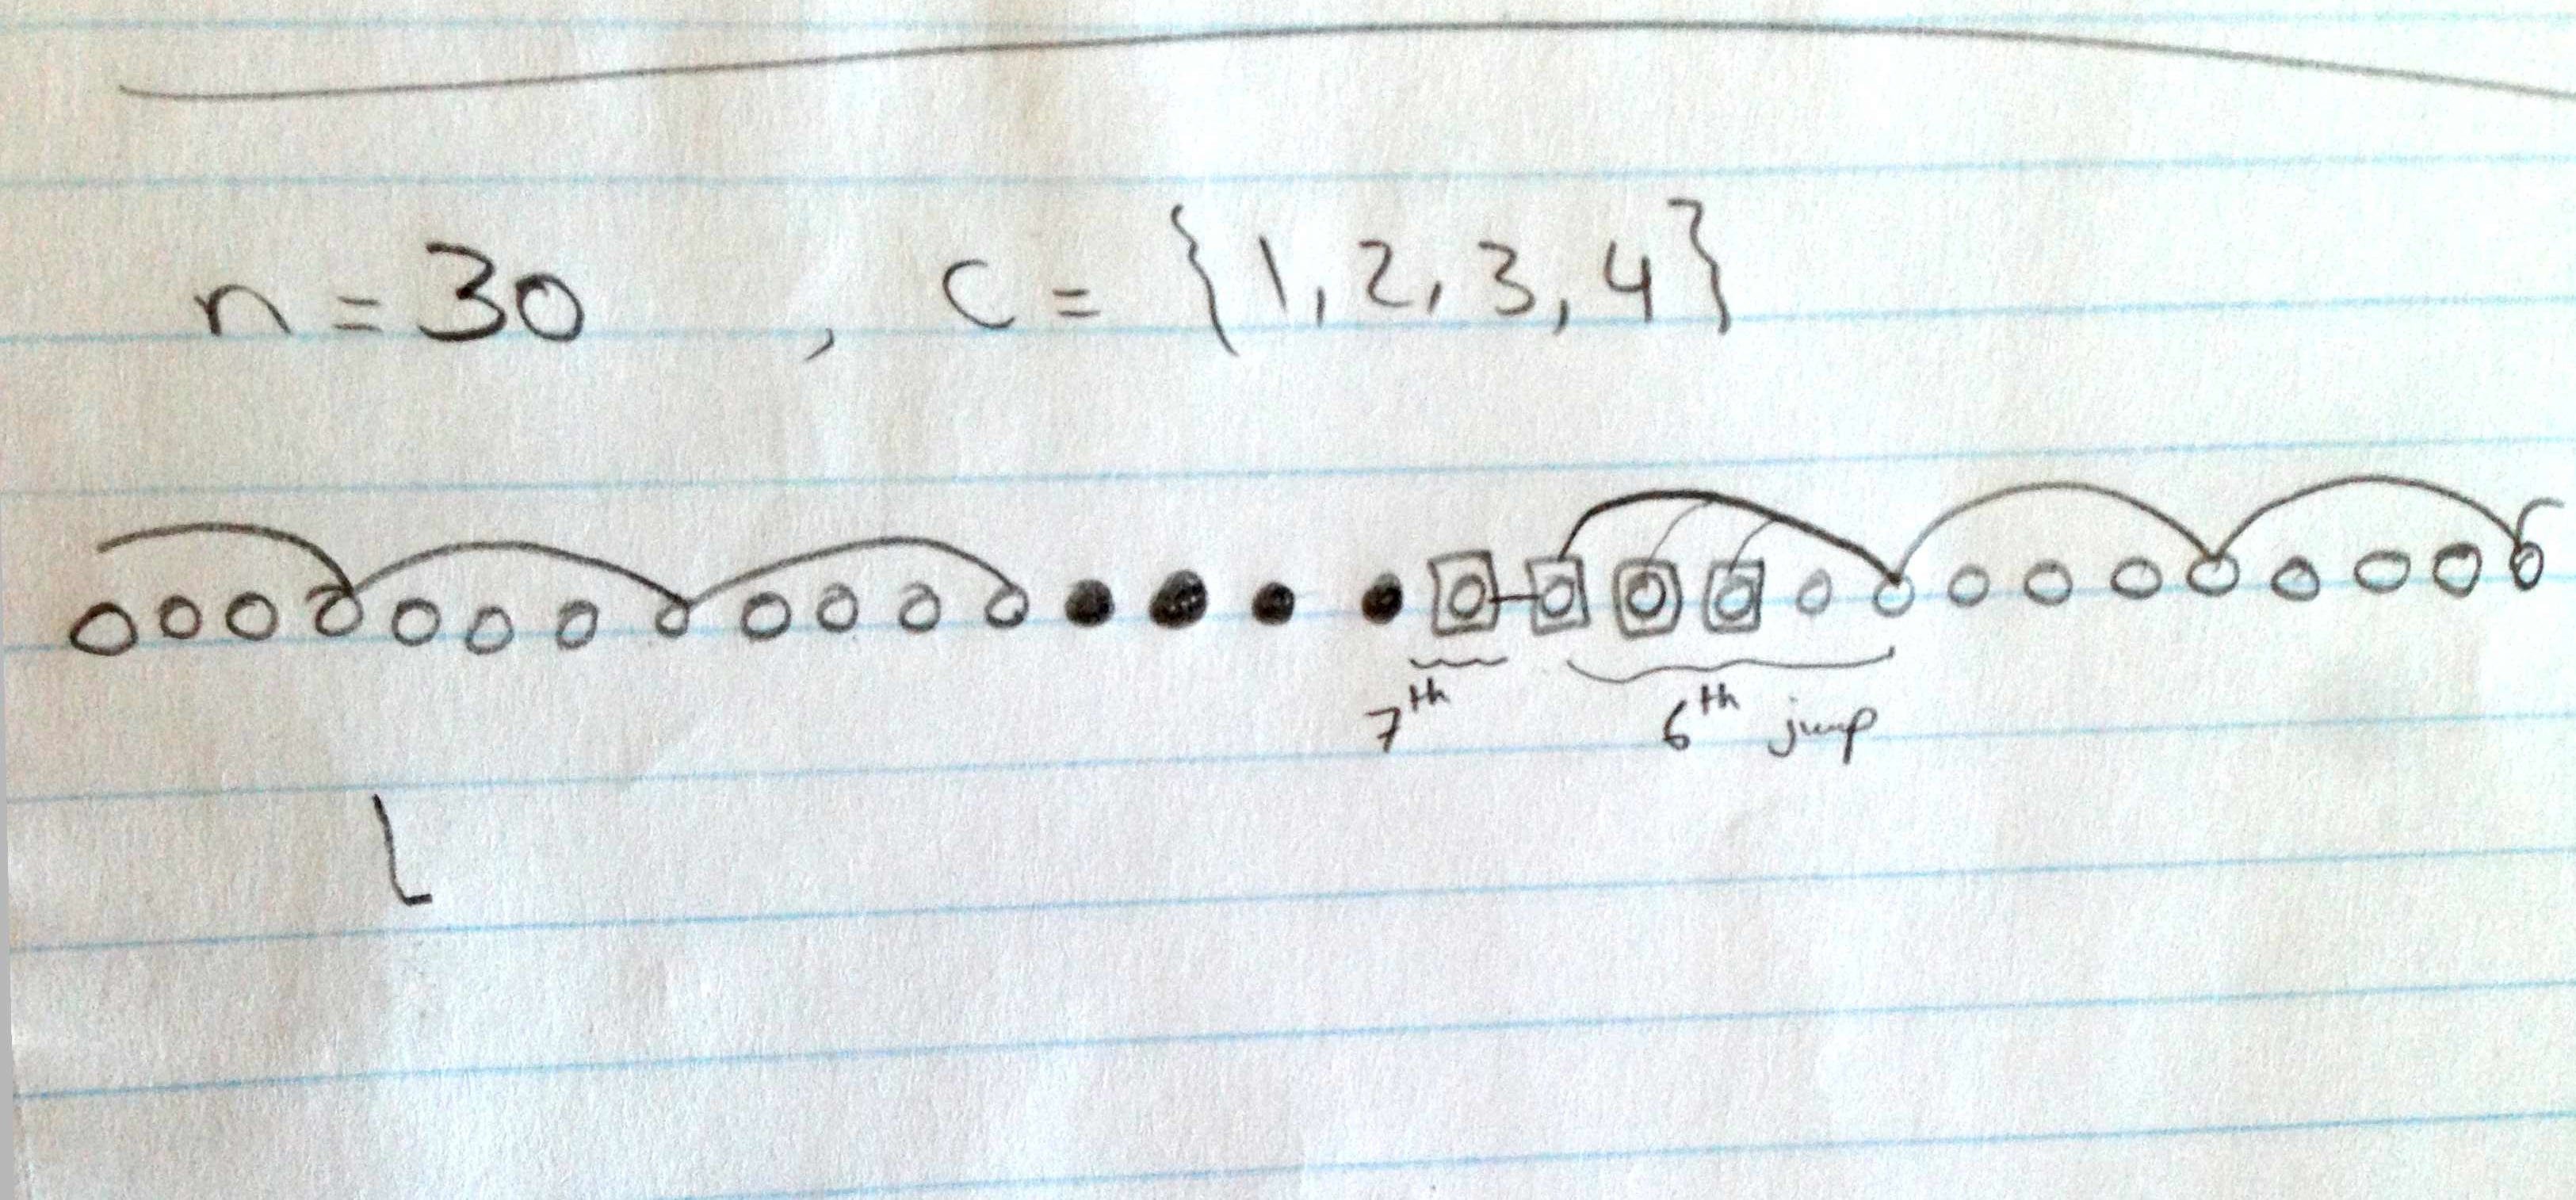
\includegraphics [scale=0.50] {consecutive.jpg}
\end {center}
\end{proof}




\begin{theorem}\label{one-d-noloop}
The  algorithm  successfully disinfects a consecutive-chord ring from \bvs in a monotone synchronous way following  the one-direction greedy strategy. 
\end{theorem}
\begin{proof}
The exploring and shadowing phase successfully locates the original \bv as demonstrated with the previous topology. It also locates the \bv in a monotone way since the maximum possible number of shadows are created at the beginning and then synchronize their movements with the exploring team. The synchronicity of our system ensures monotonicity. 
The second phase, the surrounding and eliminating phase, uses the one-direction greedy strategy and is completely free of loops since this approach forces the $SA$s to move in one direction, avoiding the \bvs in the system since the agents have knowledge of $n$ and the number and locations of $BV$s. In the first stage of this approach, $SA$ checks the number of \bvs in the system, and then moves directly through $(\lambda=-k)$ or through $(\lambda=-1)$ and then $(\lambda=-k)$. In order to ensure optimality in terms of the number of required moves, the second stage uses the simple greedy strategy to ensure a minimal distance between the target and the current location of the $SA$.

\end{proof}




\section{Conclusion }  




In this chapter, we have addressed the problem of disinfecting {\it consecutive-chord} rings from the black virus. We have demonstrated that when we have an undirected consecutive-chord ring and a synchronous execution, the exploring and shadowing phase is the same as the one employed in other topologies, having an exploring team that uses the safe exploration technique starting from the homebase and moving in a counter-clockwise direction followed by shadows until the \bv is located and triggered. We divided the outer ring into segments to demonstrate the monotone nature of our strategy. The surrounding and eliminating phase begins once the original {\it black virus} has been located. As previously mentioned, this class of chordal rings is unlike the other classes in terms of routing and directing the surrounding agents. The local strategy proposed, the {\it one-Direction Greedy}, is also a move-optimal solution. In this approach, agents must be aware of their targets and the location of the \bvs created after the activation of the original black virus. Surrounding agents traverse in a counter-clockwise direction using the edge labels to calculate their next move until they reach their targets.  We will now summarize and combine the results obtained in the previous two sections for the number of required moves.








\begin{center}
\small\addtolength{\tabcolsep}{-2pt}
\scalebox{0.7}{%

\begin{tabular}{|c|c|c|c|}\hline
{\bf $BV$ at node $v_i$} &
{\bf Phase 1} & 
{\bf Phase 2}& 
{\bf Total } 
\\ \hline\hline
$ i=1$  &$1$ & $\leq k(\lceil \frac {n-k-1}{k} \rceil) +6k-1$ & $\leq k(\lceil \frac {n-k-1}{k} \rceil) +6k$ \\\hline
$1< i<k$   &$\leq \frac{k^2+k-2}{2} -1$&$\leq k(\lceil \frac {n-k-1}{k} \rceil) +5k-1$  &$ \leq n+\frac{k^2+9k-2}{2}$  \\\hline
$k\leq i<n-k$ &$\leq (k+2)n-(\frac{3k^2+7k}{2})-3 $&  $\leq k(\lceil \frac {n-k}{k} \rceil) +2k$& $\leq ((k+3)n-(\frac{3k^2+5k}{2})$ \\\hline
$n-k\leq i<n-1$ &$\leq (k+2)n-4k-4) $& $ \leq (j-2)(\lceil \frac {n-k}{k} \rceil) +2k$ & \\ && where $j=n-|S_{area}|$ &$\leq (k+2)n-2k + (j-2)(\lceil \frac {n-k}{k} \rceil)-4)$ \\\hline
$ i=n-1$           &$(k+2)n-2k-3 $& $1$ & $\leq (k+2)n-2k-2 $ \\\hline
\end{tabular}}
\captionof{table}{Move complexity of disinfecting a consecutive-chords according to location of $BV$.}
\end{center}


The above table shows the move complexity  when we have synchronized mobile agents. The same approach can be applied using an asynchronous execution but includes an extra termination phase that can be applied by a coordinator (e.g. $LEA$). This extra phase ensures that  that  all $SA$s reach their targets before triggering the $BV$s.





